\begin{subsectionframemod}{Difference between Natural and Aerial Images}
    \metroset{block=fill}
    \begin{alertblock}{LoRA (Low-Rank Adaptation)}
        LoRA (Low-Rank Adaptation) est une technique d'optimisation qui ajuste efficacement les modèles de réseaux neuronaux de grande taille en réduisant le nombre de paramètres à ajuster via la factorisation des matrices de poids.
        En limitant le nombre de paramètres modifiés, elle aide également à réduire le risque d'overfitting tout en maintenant de bonnes performances.
    \end{alertblock}

    \only<1>{
        \begin{figure}
            \centering
            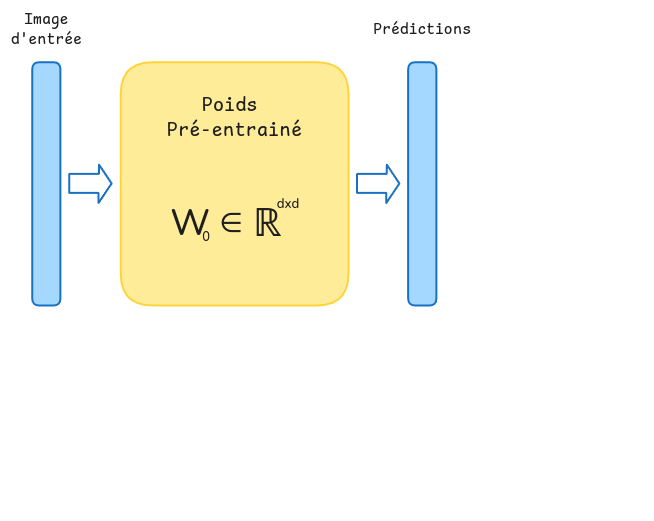
\includegraphics[width=0.6\textwidth]{Figures/lora_1}
        \end{figure}
    }
    \pause
    \only<2>{
        \begin{figure}
            \centering
            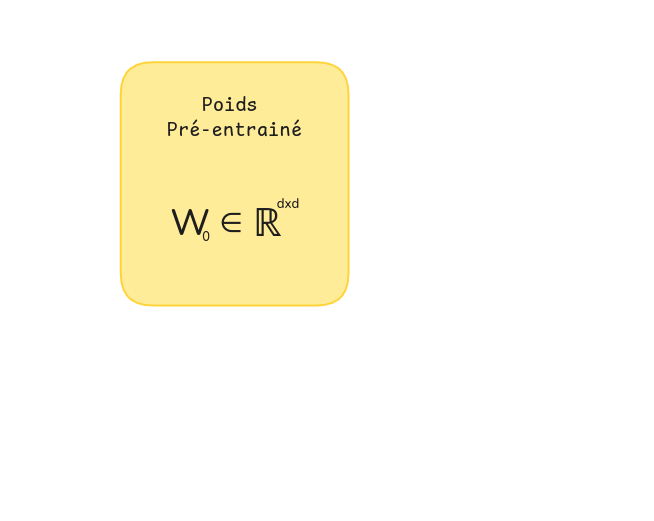
\includegraphics[width=0.6\textwidth]{Figures/lora_2}
        \end{figure}
    }
    \pause
    \only<3>{
        \begin{figure}
            \centering
            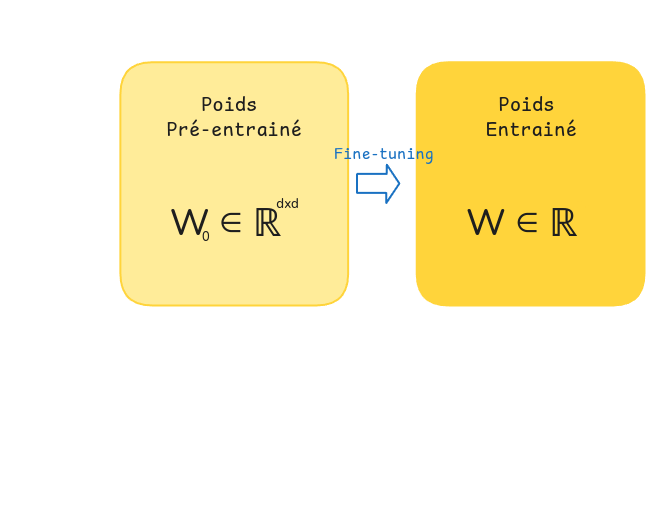
\includegraphics[width=0.6\textwidth]{Figures/lora_3}
        \end{figure}
    }
    \pause
    \only<4>{
        \begin{figure}
            \centering
            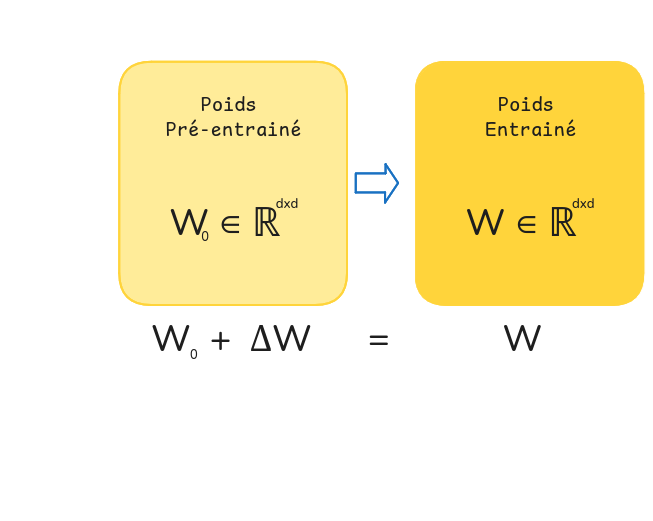
\includegraphics[width=0.6\textwidth]{Figures/lora_4}
        \end{figure}
    }
    \pause
    \only<5>{
        \begin{figure}
            \centering
            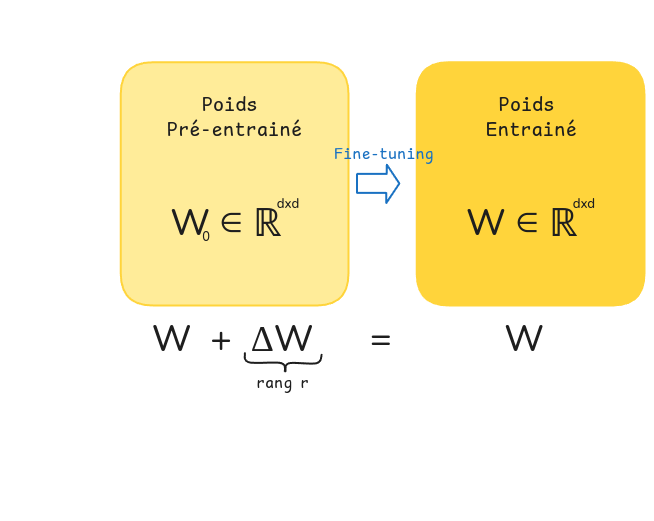
\includegraphics[width=0.6\textwidth]{Figures/lora_5}
        \end{figure}
    }
    \pause
    \only<6>{
        \begin{figure}
            \centering
            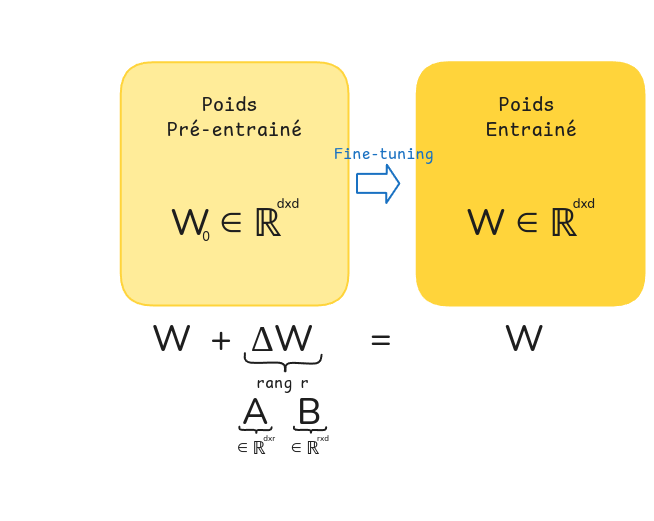
\includegraphics[width=0.6\textwidth]{Figures/lora_6}
        \end{figure}
    }


\end{subsectionframemod}